\chapter{Introduction}
\label{chap:Intro}
Just over a century has passed since Einstein first presented his work on General Relativity (GR) to the Prussian academy, ushering in a new paradigm for modern physics. In the intervening years, Einstein's remarkable theory has withstood the enormous advancements in experimental physics and observational data - with each new discovery adding further weight to this colossus of scientific endeavour. General Relativity is not only considered one of mankind's greatest scientific discoveries but one of the most significant intellectual achievements in human history. Outside of the scientific sphere, the influence of relativity can be found in the arts -- whether it be in the work of existential playwright Luigi Pirandello, who played with traditional notions of the observer, or Pablo Picasso, whose distorted perspective was reportedly inspired by the idea of displaying a fourth dimension on canvas \cite{Miller}. That is not to say, however, that Einstein's gravity does not have its shortcomings, specifically in constructing a quantum field theory of gravity; as well
as describing a viable theory of gravity, which is devoid of singularities.

String theory (ST) remains a popular candidate in formulating a consistent quantum theory of gravity \cite{polchinski1998string}, as does Loop Quantum Gravity (LQG) \cite{Ashtekar:2012np},\cite{Nicolai:2005mc}, to name just two. Whereas string theory approaches the problem rather grandly, with the intention of unifying gravity with the fundamental forces of nature, LQG makes no such claim, with the stated aim of quantizing the gravitational field. Such an approach centres around the notion of \emph{renormalisation}, in that unwanted divergences in  the  loop Feynman diagrams may be curtailed \cite{Veltman:1975vx},\cite{DeWitt:2007mi}. A third course of action can be found in the causal set programme, which considers the continuous Lorentzian manifold of GR to be an approximation of a discrete spacetime structure \cite{Henson:2006kf}. A common thread running through these fundamentally different approaches is the presence of \emph{non-locality}, where interactions occur not at a specific spatial point but over a (finite) region of space \cite{Deser:2007jk},\cite{Woodard:2014iga}\cite{Woodard:2014wia},\cite{Deser:2013uya}. Indeed, non-locality arising from infinite derivative extensions of GR has been shown to play a pivotal role in the more classical context of resolving the cosmological singularity problem, \cite{Dimitrijevic:2013ofa},\cite{Calcagni:2013vra},\cite{Dimitrijevic:2012kb},\cite{Biswas:2005qr},\cite{Biswas:2011ar}\cite{Biswas:2010zk},\cite{Conroy:2016sac},\cite{Conroy:2014dja},\cite{Chialva:2014rla}\cite{Biswas:2012bp},\cite{Craps:2014wga}, which is our focus here.

%The concept of singularities is a particularly confounding, yet intriguing, topic. Often casually referred to as a `place' where curvature `blows up', or a `hole' in the fabric of spacetime -- the concept of a singular spacetime raises thorny questions for a physicist. If a singularity is a `hole' in the fabric of spacetime, can it be  said to exist within the framework of spacetime? Could we not simply omit the singularity from our spacetime manifold? Such an interpretation would lead to a breakdown of general covariance in that the laws of physics could be amended under a simple coordinate transformation. On the other hand, if the singularity does indeed exist within the spacetime, what does it mean to have a `place' within this framework where the normal physical laws that govern the universe no longer apply? Further still, a unique characteristic of general relativity is that it is formulated without stipulating the manifold and metric structure in advance. This is in contrast to other physical theories, such as special relativity, where these are clearly defined. As such, the nature of GR means that the notion of a `place' where curvature may `blow up' is undefined a priori \cite{Geroch:1968ut},\cite{Wald:GR}. Such intuitive inconsistencies lead many to believe that singularities are not physically present in our Universe and that GR's admittance of singularities is evidence of the need to extend this powerful gravitational theory. In this way, we see the Einstein-Hilbert action of GR as a first approximation of a broader theory.

The concept of singularities is a particularly confounding, yet intriguing, topic. Often casually referred to as a `place' where curvature `blows up', or a `hole' in the fabric of spacetime -- the concept of a singular spacetime raises thorny questions for a physicist. If a singularity is a `hole' in the fabric of spacetime, can it be  said to exist within the framework of spacetime? Could we not simply omit the singularity from our spacetime manifold? On the other hand, if the singularity does indeed exist within the spacetime, what does it mean to have a `place' within this framework where the normal physical laws that govern the universe no longer apply? The difficulty lies in a unique characteristic of general relativity in that it is formulated without stipulating the manifold and metric structure in advance. This is in contrast to other physical theories, such as special relativity, where these are clearly defined. As such, without a prescribed manifold, it is not possible to discuss the concept of `outside' the manifold. Neither can one consider the notion of a `place' where curvature may `blow up' as this `place' is undefined a priori \cite{Geroch:1968ut},\cite{Wald:GR}.  Such intuitive inconsistencies lead many to believe that singularities are not physically present in our Universe and that GR's admittance of singularities is evidence of the need to extend this powerful gravitational theory. In this way, we see the Einstein-Hilbert action of GR as a first approximation of a broader theory.

Proposals for modifying general relativity have been put forward since almost its inception. Early examples include Eddington's reformulation of GR in terms of the affine connection instead of the metric tensor or Kaluza and Klein's $5$-dimensional reimagining  \cite{Clifton:2011jh}. The latter of these proposals found that the Einstein equation in $5$ dimensions yielded the $4$-dimensional Einstein field equations along with Maxwell's equations, giving hopes for a unified theory of gravitation and electromagnetism. While mathematically elegant, the Kaluza-Klein model predicted an additional massless scalar field which is in conflict with experimental data. Despite this, the technique of introducing higher dimensions is considered to be a great influence on the development of string theory \cite{zwiebach2004first}. Much later, in 1977, Stelle proposed a fourth order extension of GR \cite{Stelle:1976gc},\cite{Stelle1978}, given by
\[
{\cal L}\sim R+f_1 R^2 +f_2 R_{\mu\nu}R^{\mu\nu}+f_3 R_{\mu\nu\sigma\lambda}R^{\mu\nu\sigma\lambda}.
\] 
Fourth order or four-derivative gravity -- so-called as each term in the resulting field equations contains four derivatives of the metric tensor -- is a somewhat natural extension of gravity, if seen as a generalisation of the Gauss-Bonnet term, which appears in Lovelock gravity \cite{LovelockGB},\cite{Lovelock1969}, and is trivial in four dimensions. We return to this point briefly in Section \ref{sec:Mod}. What is remarkable, however, is that Stelle found that such theories are perturbatively renormalizable, leading to a boon in the field of quantum gravity \cite{Schmidt:2006jt},\cite{Kiefer:2012boa},\cite{Stelle:1976gc},\cite{Hamber:2007fk}. A particular instance of fourth order gravity, known as the Starobinsky model \cite{Starobinsky:1979ty}, with
\[
{\cal L}\sim R+f_0 R^2
,\]
created further interest due to its description of successful primordial inflation. Starobinsky's initial idea was to formulate a gravitational theory that mimics the behaviour of the cosmological constant. For sufficiently large $R$ this model does precisely that through the $R^2$ term, leading to the formation of the large scale structures we see in the Universe today. The quadratic curvature term becomes less dominant as the theory moves away from the Planck scale, signalling the end of inflation. 

However, finite higher derivative theories, such as fourth-order gravty, can open the door to \emph{ghosts} -- physical excitations with negative residue in the graviton propagator. This negative residue presents itself as negative kinetic energy, leading to instabilities even at a classical level \cite{Himmetoglu:2009qi}, and a breakdown in unitarity when one considers the renormalization of the theory \cite{Stelle:1976gc},\cite{Biswas:2013kla},\cite{Rubakov:2014jja}, see Chapter \ref{chap:GF} for further details.  
%Whihigher-derivative theories do not contain ghosts,  instabilities are introduced, when one considers, for example, the renormalizability of the theory 

% Even, at a classical level, ghosts, arising from finite derivative theories, can lead to a breakdown in perturbation theory, placing any predictions on shaky ground, 


Infinite derivative theories, in contrast, have the potential to describe a theory that is free of ghosts by modifying the graviton propagator via an exponent of an entire function \cite{Biswas:2005qr},\cite{Biswas:2011ar}. This exponential suppression of the propagator results in an exponential enhancement of the vertex factors of the relevant Feynman diagrams \cite{Talaganis:2016ovm}. Furthermore, the nature of this modification is such that one can always construct a modified propagator that contains no additional degrees of freedom, other than the massless graviton, so that negative residues will not propagate \cite{Biswas:2005qr},\cite{Biswas:2011ar},\cite{Biswas:2010zk},\cite{Conroy:2016sac},\cite{Conroy:2014dja},\cite{Chialva:2014rla},\cite{Biswas:2012bp},\cite{Craps:2014wga}. Infinite derivative extensions of relativity have been shown to display improved behaviour in the UV, in terms of alleviating the $1/r$ behaviour of the Newtonian potential \cite{Biswas:2011ar}, and curtailing quantum loop divergences \cite{Talaganis:2014ida},\cite{Talaganis:2015wva}. Recent progess has also been made in terms of the resolution of the black-hole singularity problem \cite{Frolov:2016pav} and a study of the dynamical degrees of freedom via Hamiltonian analysis \cite{Mazumdar:2017kxr}. Infinite derivatve extensions of relativity also allow for the formulation of non-singular cosmologies \cite{Conroy:2016sac},\cite{Conroy:2014dja}, which we cover extensively in Chapter \ref{chap:sing}, and forms the basis of the present work.  In simple terms, the \emph{objective} of this thesis is 
\begin{quote}
\emph{To present a viable extension of general relativity, which is free from cosmological singularities.}
\end{quote}
A viable cosmology, in this sense, is one that is free from ghosts, tachyons or exotic matter, while staying true to the theoretical foundations of General Relativity such as the principle of general covariance, as well as observed phenomenon such as the accelerated expansion of the universe and inflationary behaviour at later times \cite{Borde:2001nh}.

Several competing theories have been proposed as an alternative to the Big Bang model of GR. One such example is the Steady State universe. This approach is based on an extension of the cosmological principle, which imposes that the universe is homogenous and isotropic at large scales, to the \emph{Perfect} Cosmological Principle, which extends this uniformity to include time as well as space. In this sense, it conjectures that the universe has and always will exist in a state statistically similar to its current one \cite{Bondi:1948qk},\cite{Bondi:1954qj}. The steady state model, however, has suffered setbacks following the discovery of the cosmic microwave background in 1965  \cite{Weinberg:100595}, though some proponents of ``quasi-steady'' models remain \cite{Aguirre:2001ks}. 

Another popular resolution to the cosmological singularity problem is the \emph{bouncing universe} model, where the Big Bang singularity is replaced by a Big Bounce \cite{Novello:2008ra},\cite{Bozza:2005qg}. Such a cosmology issues from a scale factor that is necessarily an even function \cite{Calcagni:2013vra},\cite{Martin:2004qj}. Although the term ``Big Bounce" was not popularised until the 1980s \cite{Overduin:2006hb}, such cosmologies have a long history of interest, stretching back to the time of Willem de Sitter \cite{anderson2015cosmic}. 

Unlike bouncing models of the universe, we make no such stipulations on the nature of the cosmological scale factor a priori, preferring to confront the cosmological singularity problem by employing the Raychaudhuri equation (RE) \cite{Raych},\cite{ellis2012relativistic}, first devised in 1955 \cite{Senovilla:2014gza}. The RE is a powerful identity, which relates the geometry of spacetime to gravity, so that the behaviour of ingoing and outgoing causal geodesic congruences can be understood in a gravitational context. If these geodesics converge to a point in a finite time, they are called \emph{geodesically incomplete}, resulting in a singularity in a geometrically-flat or open cosmology \cite{Hawking:1973uf},\cite{Ellis:2003mb},\cite{Kar:2006ms},\cite{Wald:GR},\cite{Borde:1996pt},\cite{Borde:2001nh},\cite{Joshi:2013xoa}. Similarly, one can deduce the physical conditions, whereby these causal `rays' diverge, or \emph{defocus}, as a means of describing a viable non-singular cosmology. 

We will return to these points shortly, but it is perhaps instructive to first review some of the central tenets that GR relies upon - detailing what it is about GR that makes it such a special theory, before expanding on the need to modify or extend GR.
\section{General Relativity}
\label{sec:GRintro}
\emph{The Weak Equivalence Principle}\\
A key stepping stone in the formulation of GR was Einstein's Equivalence Principle, which states that, locally, inertial and gravitational mass are equivalent. Roughly speaking, this is tantamount to saying that the physics of a freely falling observer is indistinguishable from the physics of an observer in the absence of a gravitational field, which is why this principle is sometimes referred to as the \emph{universality of free fall}. In terms of Newtonian gravity, inertial mass $m_i$ is the form of mass that makes up Newton's second law of motion, i.e. $F=m_{i} a$, whereas gravitational mass $m_g$ appears in Newton's Law of Gravitation, $F=\frac{G m_{g_1}m_{g_2}}{r^2}$. The equivalence of these two forms of mass can be seen as a direct result of Galileo's leaning tower of Pisa experiment, where balls of two different masses reach the ground at the same time, in that the acceleration due to gravity is independent of the inertial or gravitational mass of the body in question. This simple insight led Einstein to formulate a theory where gravity is not described as a force but by geometry - by the curvature of spacetime \cite{Carroll:2004st},\cite{Wald:GR},\cite{Blau}.
\begin{quote}
\emph{``All uncharged, freely falling test particles follow the same trajectories once the initial position and velocity have been prescribed"} \cite{Clifton:2011jh} \\- The Weak Equivalence Principle (WEP)
\end{quote}
A fine-tuning of the Einstein Equivalence Principle led to the Weak Equivalence Principle, stated above, which has been tested rigorously over the years, beginning with the experiments of Lor{\'a}nd E{\"o}tv{\"o}s in 1908. Current experiments place the constraint on the WEP and therefore any viable relativistic theory to be
\[
\eta=2\frac{|a_1-a_2|}{|a_1+a_2|}=(0.3\pm 1.8)\times 10^{-13}
.\]
Here, beryllium and titanium were used to measure the relative difference in acceleration of the two bodies, $a_1$ and $a_2$, towards the galactic centre. This is considered to be a null result, wholly consistent with General Relativity \cite{Clifton:2011jh}.
\\\\\emph{Principle of General Covariance}\\
Another central tenet of General Relativity, which was instrumental in the formulation of GR and is perhaps more relevant to the present work, is the principle of general covariance. General covariance insists that each term making up a gravitational action will transform in a coordinate-independent way. The principle was first struck upon by Einstein when formulating the theory of special relativity, where it was proclaimed that physical laws will remain consistent in all inertial frames. Furthermore, the universal nature of the tensor transformation law offered a simple means of rendering physical equations generally covariant. That is to say that  any gravitational action expressed in terms of tensors (and covariant operators) would be a generally covariant action. Reformulating gravity in terms of tensors - with the graviton represented by a type $(2,0)$ metric tensor - allowed for a gravitational theory to be described by curvature alone. This proved to be the cornerstone of General Relativity and any valid modification or extension of GR should conform to this principle.
\\\\\emph{Gravitational Action}\\
We have now established that the central idea behind GR, as opposed to the Newtonian theory of gravitation, is that what we perceive as the force of gravity arises from the curvature of spacetime.   Mathematically, this can expressed by the gravitational action which defines the theory
\[
\label{EH}
S=\frac{1}{2}\int d^4x \sqrt{-g}\left(M_P^2 R-2\Lambda\right)
,\]
known as the Einstein-Hilbert action, where $M_P=\kappa^{-1/2}=\sqrt{\frac{\hbar c}{8\pi G}}$
%=2.435\times 10^{18}$ GeV
is the Planck mass, with $\hbar=c=1$ (natural units); $R$ is the curvature scalar, defined in Appendix \ref{sec:AppCurv}, the determinant of the metric tensor is given by $g=\det(g_{\mu\nu})$;  and  the cosmological constant is $\Lambda$, which we take to be of mass dimension $4$ in our formalism. Variation of the action with respect to the metric tensor gives rise to the famous Einstein equation
\[
\label{EinsteinEq}
M_P^2 G_{\mu\nu}+g_{\mu\nu}\Lambda= T_{\mu\nu}
,\]
where $G_{\mu\nu}\equiv R_{\mu\nu}-\frac{1}{2}g_{\mu\nu}R$ and $T_{\mu\nu}$ are the Einstein and energy-momentum tensors respectively.
%
%In terms of electrodynamics, the presence of electrodynamic fields induce a curvature in spacetime, which led to the generalisation of Maxwell's equations from a flat to a curved background. Indeed, Maxwell was particularly great inspiration for Special Relativity, when Einstein concluded that a a fixed speed of light was a direct result of Maxwell's equations [REF]. Furthermore, Kaluza and Klein showed in 192X that Maxwell's equations could be derived from a 5-dimensional theory of relativity.
%\subsection{Cosmology}
%\label{sec:introcos}
%The Friedmann-Lema\^{\i}tre-Robertson-Walker (FRW) metric forms an exact solution of Einstein's field equations and can be expressed in terms of the following isotropic and homogenous metric
%\[
%\label{FRWmetricgamma}
%ds^2=-dt^2 +a^2(t)\gamma_{ij}dx^i dx^j
%,\]
%where $\gamma_{ij}$ is a 3-dimensional  maximally symmetric metric of Gaussian curvature $k$ and the scale factor $a(t)$ is a time-dependent function of unit dimension which parametrizes the relative expansion of the Universe. To understand the geometric curvature of the spacetime more readily, it is perhaps preferable to reformulate the FRW metric in a spherically symmetric coordinate system, like so
%\[
%ds^2=-dt^2+a^2(t)\biggl(\frac{dr^2}{1-kr^2}+r^2 d\Omega^2\biggr)
%,\]
%where the spherical coordinates are contained within $d\Omega^2\equiv d\theta^2+\sin^2\theta d\varphi^2$. The spatial curvature, in terms of a hypersurface of cosmic time $t$, is given by the real constant $k$, such that
%\\
%  \begin{equation}
%    k=
%    \begin{cases}
%    -1 & \text{Negatively curved hypersurface  (Closed Universe)} \\
%      ~0 & \text{Flat hypersurface} \\
%      ~1 & \text{Positively curved hypersurface (Open Universe)}
%    \end{cases}
%  \end{equation}
%\\\emph{Exact Solution}\\  
%As the present work is largely cosmological in focus, we will now go into some detail to verify that the FRW metric is indeed an exact solution to the Einstein field equations \eqref{EinsteinEq}. In order to do this, we must derive all the relevant components that make up the metric \eqref{FRWmetricgamma}, beginning with the components of the metric tensor
%  \[
%  g_{00}=-1=g^{00},\qquad g_{ij}=a^2(t)\gamma_{ij}, \qquad g^{ij}=a^{-2}(t)\gamma^{ij}
%  .\]
%  Next, we move on to the Christoffel symbols
%  \[
%  \Gamma^\lambda_{\mu\nu}=\frac{1}{2}g^{\lambda\tau}(\partial_\mu g_{\nu\tau}+\partial_\nu g_{\mu\tau}-\partial_\tau g_{\mu\nu})
%  ,\]
%  of which the non-vanishing components are given by
%  \[
%  \Gamma^i_{0j}=\Gamma^i_{j0}=\frac{\dot{a}}{a}\delta^i_j,\qquad \Gamma^0_{ij}= a \dot{a} \gamma_{ij},
%  \]
%  where the superscript $\cdot$ denotes a derivative with respect to cosmic time. We may then use the remaining Christoffel symbols to derive the relevant forms of curvature that make up the Einstein equation, from the general definitions given in Appendix \ref{sec:AppCurv}.
%  \\\\ \emph{Ricci Tensor}\\
%  \[
%  R_{00}=-3\left(\dot{H}+H^2\right),\qquad R_{ij}=g_{ij}\left(\dot{H}+3H^2+\frac{2k}{a^2}\right)
%  \]
%\emph{Curvature Scalar}\\
%\[
%\label{FLRWscalar}
%R=6\left(\dot{H}+2H^2+\frac{k}{a^2}\right)
%.\]
%\emph{Einstein Tensor}\\
%The Einstein tensor $G_{\mu\nu}=R_{\mu\nu}-\frac{1}{2}g_{\mu\nu}R$ is then given by
%\[
%G_{00}=3\left(H^2+\frac{k}{a^2}\right),\qquad G_{ij}=-g_{ij}\left(2\dot{H}+3H^2+\frac{k}{a^2}\right),\qquad G_{0i}=0
%.\] 
%Comparing this with the Einstein Equation \eqref{EinsteinEq}, we deduce that the energy-momentum tensor must take the form
%\[
%T_{00}=\rho(t),\qquad T_{ij}=p(t)g_{ij},\qquad T_{0i}=0
%,\]
%where $\rho$ denotes the energy density and $p$ denotes the pressure. Thus, the FRW is an exact solution of Einstein's General Relativity   \cite{Carroll:2004st, Clifton:2011jh, Wald:GR, Blau}.
%\\\\ \emph{Perfect Fluid}\\
%Furthermore, this form of the energy-momentum tensor describes a \emph{pefect fluid}. A perfect fluid is one where a comoving observing views the fluid around him as isotropic. In terms of the energy-momentum tensor $T_{\mu\nu}$, isotropic spacetimes must have vanishing $T_{0i}$-components in order to remain rotationally invariant \cite{Carroll:2004st}. The remaining components are given as above, which we can express in a covariant form as follows
%\[
%T_{\mu\nu}=(\rho+p)u_\mu u_\nu +p g_{\mu\nu}
%.\]
%Here, $u_\mu$ is the fluid four-velocity, i.e. $u_{\mu}=\{1,0,0,0\}$, such that $g^{\mu\nu}u_\mu u_\nu=-1$ and $(u^\mu k^\mu)^2=(k^0)^2$. We then perform the operations of (1) contracting with this fluid four velocity, (2) contracting with the \emph{null} geodesic congruence $k^\mu$ and (3) taking the trace to express three distinct identities:
%\[
%\label{Tu}
%T_{\mu\nu}u^\mu u^\nu=\rho 
%\]
%\[
%\label{Tk}
%T_{\mu\nu}k^\mu k^\nu=(\rho+p)(k^0)^2
%\]
%\[
%\label{Ttrace}
%T=-\rho+3p
%.\]
%Next, we note that combining the conditions $T_{\mu\nu}u^\mu u^\nu\geq 0$ and $T_{\mu\nu}k^\mu k^\nu\geq0$ implies $T_{\mu\nu}\xi^\mu \xi^\nu\geq 0$, where $\xi^\mu$ denotes a \emph{timelike} geodesic congruence, which is precisely the \emph{Weak Energy Condition} (WEC). The WEC states that the energy density will be positive for an observer along a timelike tangent vector $\xi^\mu$. The null energy condition (NEC), given by $T_{\mu\nu}k^\mu k^\nu$, is a special case of the WEC, where the timelike tangent vector is replaced by a null ray. In this case, the energy density may conceivably be negative so long as this is balanced by sufficiently positive pressure. In terms of the perfect fluid, these are given by 
%\begin{itemize}
%\item {\bf Null Energy Condition:}
% $T_{\mu\nu}k^\mu k^\nu\geq 0$ implies $\rho+p\geq0$ \label{NEC}
%\item {\bf Weak Energy Condition:} $T_{\mu\nu}\xi^\mu \xi^\nu\geq 0$ implies $\rho+p\geq0$ and $\rho\geq0$ \cite{Carroll:2004st}.
%\end{itemize}
%The NEC, in particular, will play an important role in the later discussion on singularity-free theories of gravity in Chapter \ref{chap:sing}. 
\section{Modifying General Relativity}
Despite the phenomenal success of the theory of relativity, outstanding issues remain, which suggests that the theory is incomplete. As mentioned in the introduction, one of these issues concerns the construction of a theory which marries  quantum field theory (QFT) with GR. This has been an open question in modern physics since almost the inception of QFT in the 1920s, but gained particular traction with the rise of string theory in the 1960s and 70s.
% Much of the recent investigation in to quantum gravity centres around the idea of constructing a gravitational theory that is \emph{renormalizable}, in that unwanted divergences in the loop Feynmann diagrams may be brought to heel. Attacking the problem in this manner forms the basis for Loop Quantum Gravity, where non-locality plays a pivotal role. 
A more classical shortcoming of GR arises from its admittance of singularities, where the normal laws of physics can be said to `break down'. We now discuss how GR cannot describe a viable, non-singular cosmology, in order to motivate the need to extend the theory.
\\\\ \emph{Singularities}\\
The Cosmological Singularity Problem is the focal point of the present text, with Chapter \ref{chap:sing} devoted to the description of a stable, \emph{extended} theory of relativity devoid of an initial singularity. The requirement of extending GR in order to avoid a Big Bang singularity can be seen by referring to the Raychaudhuri equation (RE), see Section \eqref{sec:RE} for full details. The RE is a powerful identity which relates the geometry of spacetime to gravity, so that the behaviour of ingoing and outgoing causal geodesic congruences can be understood in a gravitational context. From this, one can deduce the necessary conditions whereby ingoing causal geodesics will converge to the same event in a finite time. This convergence is known as \emph{geodesic incompleteness} and a freely falling particle travelling along this geodesic will, at some finite point in time, cease to exist. We call such a spacetime \emph{singular} and the associated condition is known as the \emph{convergence condition} \cite{Geroch:1968ut}. 

Here, we merely outline the convergence conditions in GR, which are discussed in greater detail in Chapter \ref{chap:sing}, as a means of motivating the need to modify or extend the theory. From the RE, one can deduce that a spacetime will be null-geodesically incomplete if either of the following conditions are met \cite{Kar:2006ms},\cite{Borde:1996pt},\cite{Vachaspati:1998dy},
\[
\frac{d\theta}{d\lambda}+\frac{1}{2}\theta^2\leqq 0,\qquad R_{\mu\nu}k^\mu k^\nu\geq 0.
\]
Leaving aside the left hand inequality for the moment, which describes the convergence condition in terms of geometric expansion, let us focus on the right hand inequality within the framework of GR. From the Einstein-Hilbert action \eqref{EH}, we derive the Einstein equation \eqref{EinsteinEq}, while also noting that null geodesic congruences vanish when contracted with the metric tensor, according to $g_{\mu\nu}k^{\mu}k^{\nu}=0$. Thus,
\[
R_{\mu\nu}k^\mu k^\nu = \kappa T_{\mu\nu}k^\mu k^\nu 
,\]
must be positive in order to retain the null energy condition (NEC), see Appendix \eqref{NEC}, and to avoid the propagation of potentially exotic matter \cite{Capozziello:2013vna},\cite{Elder:2013gya}. Thus, in GR we are left with the choice of either accepting singularities or accepting potentially non-physical matter. As neither option is desirable, we conclude that GR must be extended in order to describe a viable non-singular cosmology.
\\\\\emph{Lovelock's Theorem}\\
An important theorem in both the formulation of GR and concerning any valid extension of the theory is \emph{Lovelock's Theorem}\cite{Clifton:2011jh},\cite{Lovelock1969}
\begin{theorem}[Lovelock's Theorem]
The only possible \emph{second-order} Euler-Lagrange expression obtainable in a four-dimensional space from a scalar density with a Lagrangian dependent on the metric tensor (i.e. ${\cal L}={\cal L}(g_{\mu\nu})$) is
\[
E^{\mu\nu}=\sqrt{-g}\left(\alpha G^{\mu\nu}+g^{\mu\nu}\lambda\right),
\]
where both $\alpha$ and $\lambda$ are constants 
\end{theorem}
 This is a remarkable result when one considers that by taking $\lambda=\Lambda$, this is precisely the Einstein equation in the presence of the cosmological constant, modified only by the constant $\alpha$. What this theorem says is that any gravitational theory in a four-dimensional Riemannian space, whose subsequent field equations are of second order or less will be defined solely by the Einstein equation. As we have seen, the Einstein Hilbert action \eqref{EH} produces the the Einstein field equations \eqref{EinsteinEq} precisely, but a more general action does exist (in four dimensions) that also reproduces the same result, and this is given by
 \[
 \label{EHgen}
 {\cal L}=\sqrt{-g}\left(\alpha R-2\Lambda\right)+\beta\sqrt{-g}\left(R^2-4R^{\mu\nu}R_{\mu\nu}+R^{\mu\nu\lambda\sigma}R_{\mu\nu\lambda\sigma}\right)+\gamma\epsilon^{\mu\nu\lambda\sigma}R^{\alpha\beta}{ }{ }_{\mu\nu}R_{\alpha\beta\lambda\sigma}
 .\]
 In four dimensions the final two terms do not contribute to the field equations. Whereas this is true for the final term in any number of dimensions, the second term is what as known as the Gauss Bonnet term and is non-trivial in theories of dimensions higher than four.

What Lovelock's theorem means for modified theories of gravity is that, if we assume that we want to describe a generally covariant, four-dimensional, metric-tensor-based theory of gravity, whilst retaining the variational principle, we have two options: 
\begin{enumerate}
\item[1.] Extend our approach into field equations that contain higher than second order derivatives and/or 
\item[2.] Allow a degree of non-locality to enter the system.\cite{Clifton:2011jh}
\end{enumerate}
\leavevmode

\subsection*{Examples of Modified Theories}
\label{sec:Mod}
\emph{Fourth Order Gravity}\\
We have already noted that the action \eqref{EHgen} is the most general action that reproduces the Einstein-field equation. A generalisation of the Gauss-Bonnet term
\[
G_{GB}=R^2-4R^{\mu\nu}R_{\mu\nu}+R^{\mu\nu\lambda\sigma}R_{\mu\nu\lambda\sigma},
\]
forms the basis for what is called \emph{Fourth Order Gravity},
\[
{\cal L}=R+f_1 R^2 +f_2 R_{\mu\nu}R^{\mu\nu}+f_3 R_{\mu\nu\sigma\lambda}R^{\mu\nu\sigma\lambda}.
\]
As stated in the introduction, Stelle observed that fourth order theories were perturbatively renormalisable, leading to a great generation of interest in quantum gravity \cite{Stelle:1976gc}. However, such theories are beset by the presence of ghosts, see Section \ref{sec:patho} for further details.
\\\\\emph{$f(R)$-gravity}\\
Perhaps the simplest generalisation of the Einstein-Hilbert action \eqref{EH} comes in the form of $f(R)$-gravity, where the curvature scalar $R$ is replaced by an arbitrary function $f$ acting on the curvature $R$,
\[
S=\frac{M_P^2}{2}\int d^4x \sqrt{-g} f(R)
.\]
By varying with respect to the metric tensor, we can then read off the $f(R)$ field equations
\[
\kappa T_{\mu\nu}=f^{\prime}(R)R_{\mu\nu}-\frac{1}{2}g_{\mu\nu}f(R)+g_{\mu\nu}\square f'(R)-\nabla_{\mu}\nabla_{\nu}f^{\prime}(R),\]
where $f^{\prime}=\partial f(R)/\partial R$, $\Box=g^{\mu\nu}\nabla_\mu\nabla_\nu$ and using $\delta f(R)=f'(R)\delta R$.
\\\\ \emph{Starobinsky Model}\\
The Starobinsky model is a particular instance of $f(R)$-gravity with
\[
f(R)=R+c_0 R^2
,\]
for some real constant $c_0$. Recall that Starobinsky's initial idea was to formulate a gravitational theory that mimics the behaviour of the cosmological constant, leading to successful primordial inflation. This model will be of particular interest when discussing the defocusing conditions of infinite derivative theory, where it is found that the Starobinsky model struggles to pair successful inflation with the avoidance of singularities. See Section \ref{sec:defocusmink}.
\section{Infinite Derivative Theory of Gravity}
\label{sec:IDGintro}
The most general infinite derivative action of gravity that is quadratic in curvature was first derived in \cite{Biswas:2005qr}, and was found to take the form
\[
\label{actionint}
S=\int d^4x\frac{\sqrt{-g}}{2}\left[M_P^2R+ \lambda R{\cal F}_1(\Box)R
+\lambda R_{\mu\nu} {\cal F}_2(\Box)R^{\mu\nu}
+\lambda C_{\mu\nu\lambda\sigma} {\cal F}_{3}(\Box)C^{\mu\nu\lambda\sigma}\right],
\]
where the form factors ${\cal F}_i(\Box)$ are given by
\[
{\cal F}_i(\Box)=\sum^{\infty}_{n=0}f_{i_n}\left(\Box/M\right)^n
\]
and $M$ is the scale of non-locality. 
In this form, we can see this as a natural generalisation of fourth order gravity to include all potential covariant operators in accordance with the principle of general covariance.
The above action has been studied extensively in terms of the modified propagator \cite{Biswas:2013kla}; Newtonian potential \cite{Edholm:2016hbt},\cite{Biswas:2011ar}; gravitational entropy \cite{Conroy:2015wfa},\cite{Conroy:2015nva}; loop quantum gravity \cite{Talaganis:2014ida},\cite{Talaganis:2015wva},\cite{Talaganis:2016ovm}; and indeed, singularity avoidance \cite{Conroy:2016sac},\cite{Conroy:2014dja},\cite{Frolov:2016pav}. We will summarise some relevant results shortly. Firstly, however, let us briefly expand on the notion of non-locality, alluded to in the introductory paragraphs.
\\\\\emph{Non-locality} \\
We stated earlier that a consequence of Lovelock's theorem is that a valid modified theory of gravity must include derivatives that are of second order or higher and/or allow a degree of non-locality. In this sense, the action \eqref{actionint} conforms to both of Lovelock's stipulations in that it is both of higher order than 2 and non-local, so that \eqref{actionint} can be understood as an effective action \cite{Biswas:2005qr},\cite{Barvinsky:2002uf}.  A theory featuring an \emph{infinite series of higher-derivative} terms, such as the infinite derivative gravity (IDG) theory introduced above, and derived in Chapter \ref{chap:2}, yields non-local interactions and a relaxation of the principle of locality, which, in simple terms, states that a particle may only be directly influenced by its immediate surroundings.

The quantum interactions of these infinite derivative terms have been studied and found to potentially alleviate divergences in the UV, by allowing for the super-renormalizability of the theory \cite{Tomboulis:1997gg},\cite{Moffat:2010bh},\cite{Talaganis:2014ida}. Non-local objects, such as strings and branes, are a fundamental  component of string theory, while the formulation of Loop Quantum Gravity is based on non-local objects, such as Wilson Loops \cite{Talaganis:2015wva}. The IDG theory, defined by the action \eqref{actionint} was inspired by the non-locality that arises from  exponential kinetic corrections, common in string theory, see \cite{Biswas:2005qr},\cite{zwiebach2004first}. In terms of the Feynman diagrams, non-local interactions result in an exponential enhancement of the vertex operator, meaning that interaction does not take place at this point, as in a local theory \cite{Talaganis:2014ida, Stelle:1976gc, Goroff:1985th}. 
Note also, that while a series of infinite derivatives is a common feature of non-local theories, it is not true to say that this is a defining characteristic. For example, massive gravity theories which modify GR in the infrared, e.g. $\sim \frac{1}{\Box^2} R$, are indeed non-local but have finite orders of the inverse D'Alembertian \cite{Maggiore:2013mea},\cite{Maggiore:2014sia},\cite{Conroy:2014eja},\cite{Jaccard:2013gla},\cite{Modesto:2013jea}.

\subsection*{Summary of Results}
In this section, we summarise some of relevant results, achieved within an infinite derivative gravitational framework, that are not explicitly covered in the subsequent chapters.\\\\
\emph{Newtonian Potential}\\
In \cite{Biswas:2011ar}, the Newtonian potential was studied around the weak field limit of the action \eqref{actionint}. In this case, the modified propagator was modulated by an overall factor of  $a(\Box)=e^{-\Box/M^2}$, where $M$ is the scale of modification. The exponential nature of this function was invoked in order to render the theory ghost and tachyon free, which is covered in detail in Chapter \ref{chap:GF}. For a theory with modified propagator $\Pi$, given by
\[
\Pi=\frac{1}{a(-k^2)}\Pi_{GR}
,\]
where $\Pi_{GR}$ is the physical graviton propagator and $\Box\rightarrow -k^2$ in Fourier space on a flat background, the Newtonian potential $\Phi(r)$ was found to be
\[
\label{erf}
\Phi(r)\sim\frac{m\pi}{2M_P^2 r}\mbox{Erf}(\frac{r M}{2})
.\]
Here, we observe that the potential contains the familiar $1/r$ divergence of GR, modulated by an error function Erf$(r)$. At the limit $r\rightarrow \infty$ \footnote{Alternatively, if we take $M\rightarrow\infty$, which is the limit to return IDG to a local theory, we recapture the familiar $1/r$ divergence of GR, as expected.}, $\mbox{erf}(r)/r\rightarrow 0$ returning flat space. Furthermore. at the limit $r\rightarrow 0$, the potential converges to a constant, thus ameliorating the $1/r$ drop-off of GR and displaying improved behaviour in the UV. The explicit calculation  can be found in Appendix \ref{chap:NewtPot}. The behaviour of the Newtonian potential in an IDG theory was further expanded upon in \cite{Edholm:2016hbt}, where a more general ghost-free form factor
\[
a(\Box)=e^{-\gamma(\Box/M^2)}
\]
was studied, where $\gamma$ is some entire function. In this case, identical limits were observed at $r\rightarrow \infty$. Furthermore, using laboratory data on the gravitational potential between two masses at very small distances, the lower limit $M>0.004eV$ was placed on the the scale of modification.
\begin{figure}[h]
\centering
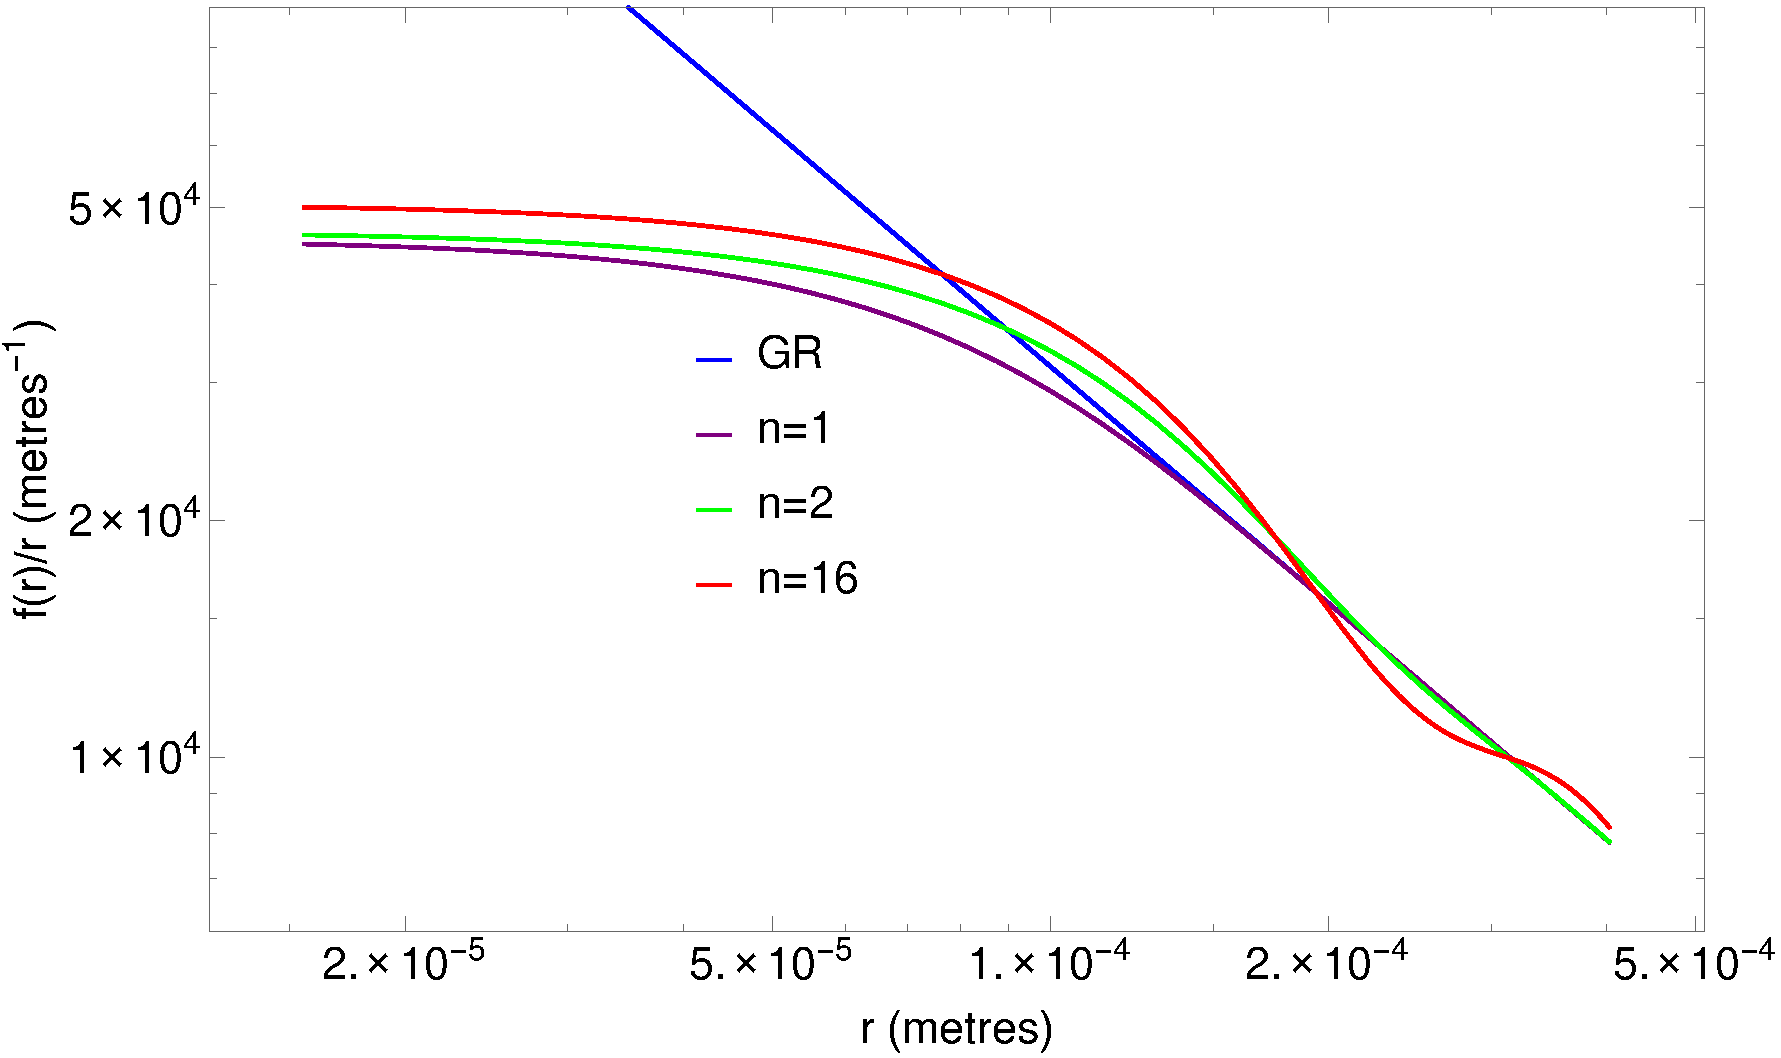
\includegraphics[scale=0.4]{monomialgraph.pdf}\cite{Edholm:2016hbt}
\caption{A plot of the Newtonian potential $\Phi(r)\sim f(r)/r$ vs. $r$ where $n=1$ corresponds to \eqref{erf} with $a(\Box)=e^{-\Box/M^2}$. Higher orders of $n$ are given by the exponential modification $a(\Box)=e^{-(\Box/M^2)^n}$, where $M$ has been taken to be the value of the lower bound, $M=0.004$eV for illustrative purposes} 
\end{figure}
\\\\\emph{Entropy}\\
The gravitational Wald entropy for IDG theories was investigated across two papers in \cite{Conroy:2015wfa} and \cite{Conroy:2015nva}. It was found in \cite{Conroy:2015wfa} that the gravitational entropy accounting for the UV-modified
sector vanishes around an axisymmetric black-hole metric when one requires that no additional degrees of freedom are introduced in the linear regime -- a condition which results in a ghost-free theory. The
resulting entropy was given simply by the famous area law, 
\[
S_{\text{\it Wald}}=\frac{\mbox{Area}}{4G}
.\]
%The result was a surprising one, leading us to conjecture that non-local modifications were the ground state of the graviton. 
In \cite{Conroy:2015nva}, the analysis was extended to consider the gravitational entropy around an (A)dS metric, where a lower bound on the leading order modification term was calculated which precludes non-physical spacetimes characterised by negative entropy. This bound was found to have cosmological significance in terms of avoiding singularities around a linearised de Sitter background. See Section \ref{sec:Entropy} for an outline of this result.
\\\\\emph{Quantum Loop Gravity}\\
Quantum aspects have been studied for  IDG theories, specifically from the point of view of a toy model, see \cite{Talaganis:2014ida}. Here,  explicit 1-loop and 2-loop computations were performed where it was found that, at 1-loop, a divergence arises. However, counter terms can be introduced to remove this divergence, in a similar fashion to loop computations in GR. Furthermore, at 2-loops the theory becomes finite. The article \cite{Talaganis:2014ida} then suggests a method for rendering arbitrary n-loops finite.
\\\\\emph{Modifications in the Infrared}\\\begin{figure}[h]
\centering
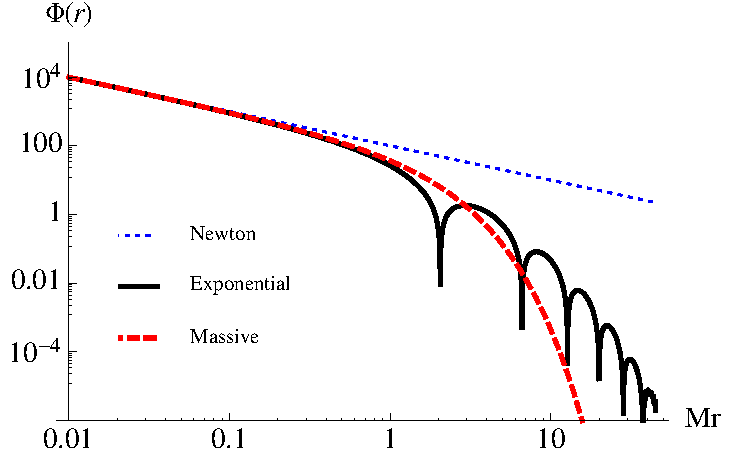
\includegraphics[scale=0.8]{IRpotentials.pdf}
\caption{Plot showing the suppression of the gravitational potential in the exponential model. The thick black line is the potential of the exponential model. Few initial oscillations are visible as the potential is suppressed with respect to the Newtonian 1/r behaviour depicted by the thin blue dotted line. For comparison, we also show the pure Yukawa suppression of massive gravity as the dashed red line.} 
\end{figure}The present work focuses solely on modifications to GR in the UV. Recently, however, interest has been generated in the field of non-local modifications in the infrared (IR). Such theories are characterised by the presence of inverse D'Alembertian ($1/\Box$) corrections in the gravitational action. Most notably, recent work has centred on the idea of constructing a theory of gravity which confers a non-zero mass upon the graviton, known as \emph{massive gravity}. Massive gravity theories are formulated via a $\frac{m_{gr}^2}{\Box^{2}}R$ -type extension to the Einstein-Hilbert action, where $m_{gr}$ is the mass of the massive graviton. Such theories have been explored in a number of papers as a means to explain the proliferation of dark energy in the Universe \cite{Maggiore:2013mea},\cite{Maggiore:2014sia},\cite{Modesto:2013jea},\cite{Jaccard:2013gla},\cite{Dirian:2014ara}\cite{Dirian:2014xoa}. 

In \cite{Conroy:2014eja}, the full non-linear field equations for a generalised action made up of an infinite series of inverse D'Alembertian operators was derived for the first time. The gravitational action can be formulated by replacing the form factors ${\cal F}_i(\Box)$ in \eqref{actionint} with
\[
{\cal {\bar F}}_i(\Box)=\sum_{n=1}^{\infty} f_{-n}(M^2/\Box)^n
.\]
Similar methods to \cite{Biswas:2011ar} were employed in order to derive the modified Newtonian potentials, with the added complexity that models with an additional degree of freedom in the scalar propagating mode were not excluded, i.e. $a\neq c$ in Appendix \ref{chap:NewtPot}, resulting in two Newtonian potentials. An upper bound was placed on the ratio of these potentials, known as the Eddington parameter, via the Cassini tracking experiment and various models were analysed as a means of explaining dark energy, including $Rf(R/\Box)$-models \cite{Deser:2007jk} and massive gravity. In the context of massive gravity, the massive graviton was tested and found to fall within the appropriate limits to be considered a possible dark energy candidate. Finally, a novel approach to infrared modifications was introduced, making use of all infinite inverse derivatives, which displayed a reduction in the gravitational field at large distances -- a common feature of IR extensions to GR.  
\newpage
\section{Organisation of Thesis}
The content of the thesis is organised as follows:
\begin{enumerate}
\item[Chapter 2:] This chapter begins with a derivation of the most general, generally covariant, infinite derivative action of gravity that is quadratic in curvature, before moving on to the main focus of the chapter: the highly non-trivial task of attaining the full non-linear field equations. The general methodology is outlined before moving on to the explicit calculation. Finally the linearised field equations are derived around both Minkowski and de Sitter spacetimes for later use in the context of ghost and singularity free cosmologies.

\item[Chapter 3:] The general ghost and tachyon criteria that a viable theory must conform to are established, with specific examples of pathological behaviour  given. The correction to the graviton propagator from the infinite derivative extension is attained, as are the ghost-free conditions around Minkowski space.

\item[Chapter 4:] This final chapter is the crux of the thesis, combining the field equations (Chapter 2) and the ghost-free conditions (Chapter 3) to formulate a viable singularity-free theory of gravity. The chapter begins with a discussion on the intriguing topic of defining a singularity, before moving on to an outline of the famous Hawking-Penrose Singularity Theorem. The Raychaudhuri equation (RE) is introduced and derived, with particular attention paid to the RE in a cosmological setting. A novel calculation then follows where the RE is applied to infinite derivative gravity theory and viable \emph{defocusing conditions} are derived around Minkowski and de Sitter spacetimes.
\end{enumerate}